
\chapter{Planning-based Approach in Details}

\label{Chapter4} % For referencing the chapter elsewhere, use \ref{Chapter1} 

\section{Full Implementation Details}

\subsection{Environment Description}
The environment used to test this approach is a fighting game we created called \textit{FG}. This gave us complete control over the dynamics of the game. It also gave us access to internal game data which would have been considerably more difficult to access had we instead opted to modify an existing fighting game. 

The game is structured as a traditional fighting game. Players move back and forth on in a 2D space, trying to land blows on one another to reduce the opponents health to zero. There are a total of 21 types of actions that the player can perform, and each of these actions can be done for a duration that corresponds to some number of frames. The specific types of actions that players can take are described in Table \ref{actions}.

The state of the game is represented by a combination of the states of the player and opponent. A player's state includes its world position in discretized space, an indicator of its velocity, and its current status. Details are described in Table \ref{gamestate} and Table \ref{playerstatus}




%Old Stuff from Previous Drafts
%In order to perform search, we need a way to generate the successors of state $s$. Specifically, we need a way to generate $s' = succ(s, a)$ where $a$ is an action defined by a type and a duration. Because we don't actually know the full dynamics of the game, we extract them from the player's demonstration.


%An issue that still is prevalent is that of robustness. When the AI encounters a state that it hasn't seen before, what should it do? We propose to solve this issue using a technique we dub \textbf{action effects}. The idea is that many actions have easily predictable actions. For example, moving left for a long time will always move the player a certain distance to the left. This formulation works for this domain because the results of actions in fighting games are completely predictable, as it's all codified inside the game engine. 

%What does one do with these action effects? Well, we can use them to give the AI an idea of what to do in a state it hasn't seen before

%\begin{figure}[t]
%	\centering
%	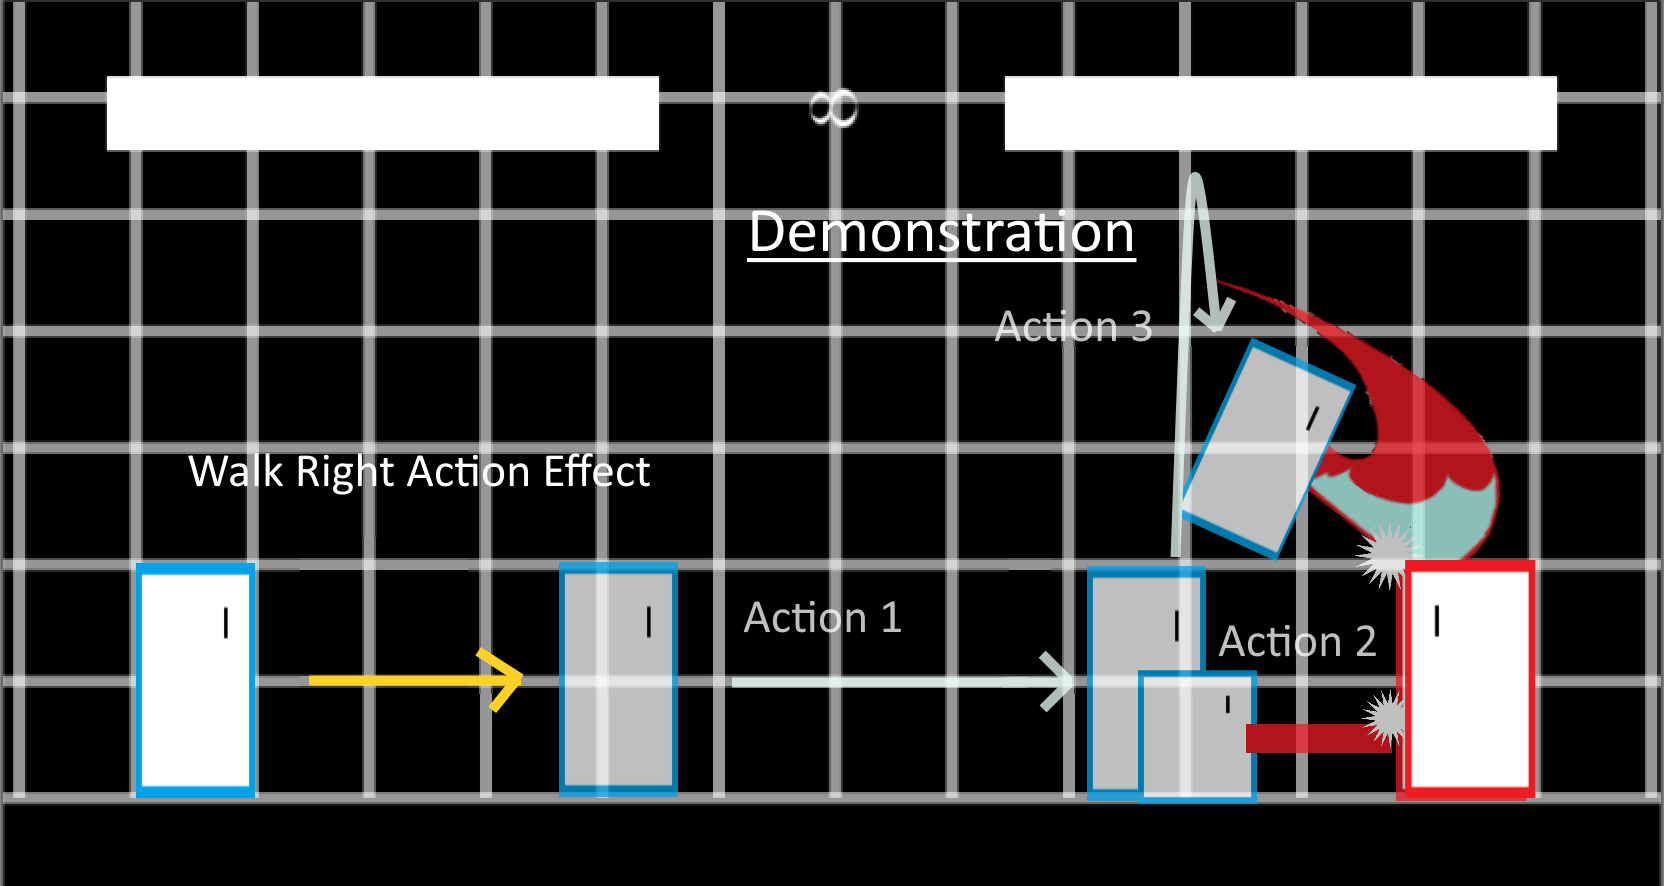
\includegraphics[width=\textwidth]{Figures/ActionEffect.png}
%	\caption{Action Effects}
%	\label{ActionEffects}
%\end{figure}


%For example, lets say that the player starts from far away from the demonstration etc etc.


%\section{Algorithm Design and implementation}

%In order to formulate the fighting game as a search problem, we need to discretize the state space as a graph. The nodes on this graph represent the game state at a specific point in time. This includes the positions of the players, their velocities, and various other metrics that capture their internal state. Full details can be found in Table \ref{gamestate}. The edges between nodes $a$ and $b$ represent transitioning from state $a$ to state $b$ via a \textbf{preformed action}. These are tuples which dictate an \textbf{type} of action that a player can perform and a \textbf{duration} that it is performed for. The set of actions that the AI can perform is restricted to the actions performed by the player in the training data. 

%\subsection{Extracting game dynamics}

\subsection{Data Extracted from Demonstration}

In order for the AI to generate plans, we need a human demonstration to build a model of the game dynamics. Throughout this section, we will refer to a simple human demonstration where the player moves forward, hits the opponent with a low attack, and then jumps to hit the player with a jumping attack.

\begin{figure}[h]
	\centering
	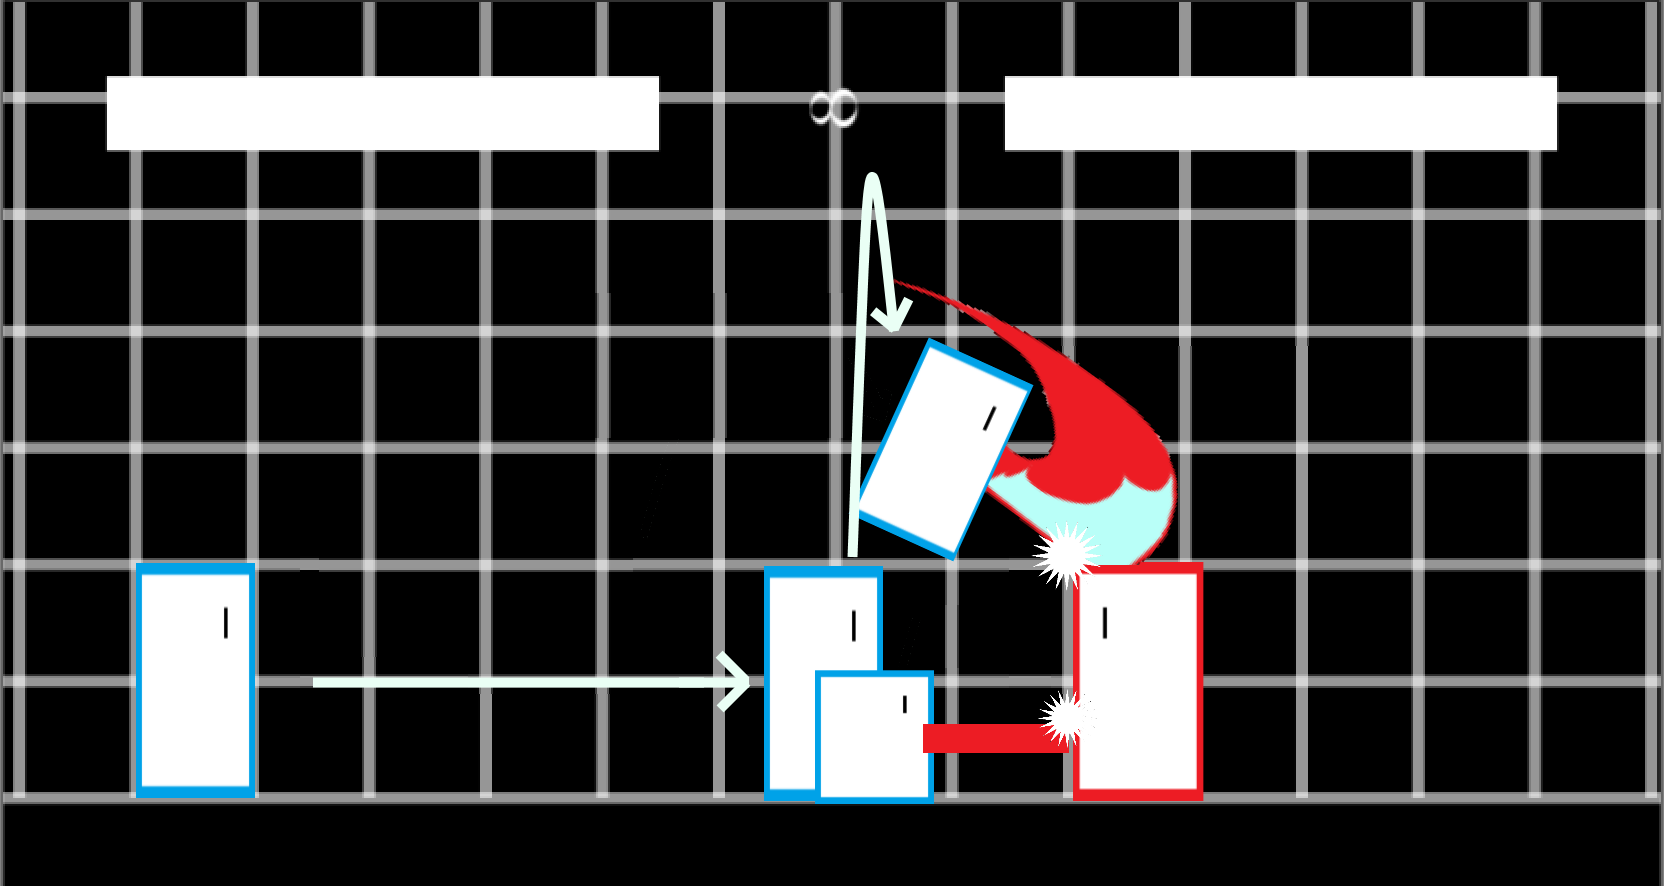
\includegraphics[scale=0.5]{Figures/Demonstration.png}
	\caption{A Time lapse of the demonstration}
	\label{ActionEffects}
\end{figure}

As the demonstration plays out, the target player performs actions to transition between different game states. A transition $(s,a,s')$ is recorded in each of the following cases

1. When the player starts performing a new action

2. When the player is hit during the current action, ending it early. 

3. When the game state changes during the current action.

\begin{figure}[h]
	\centering
	\begin{subfigure}[h]{0.3\textwidth}
		\centering
		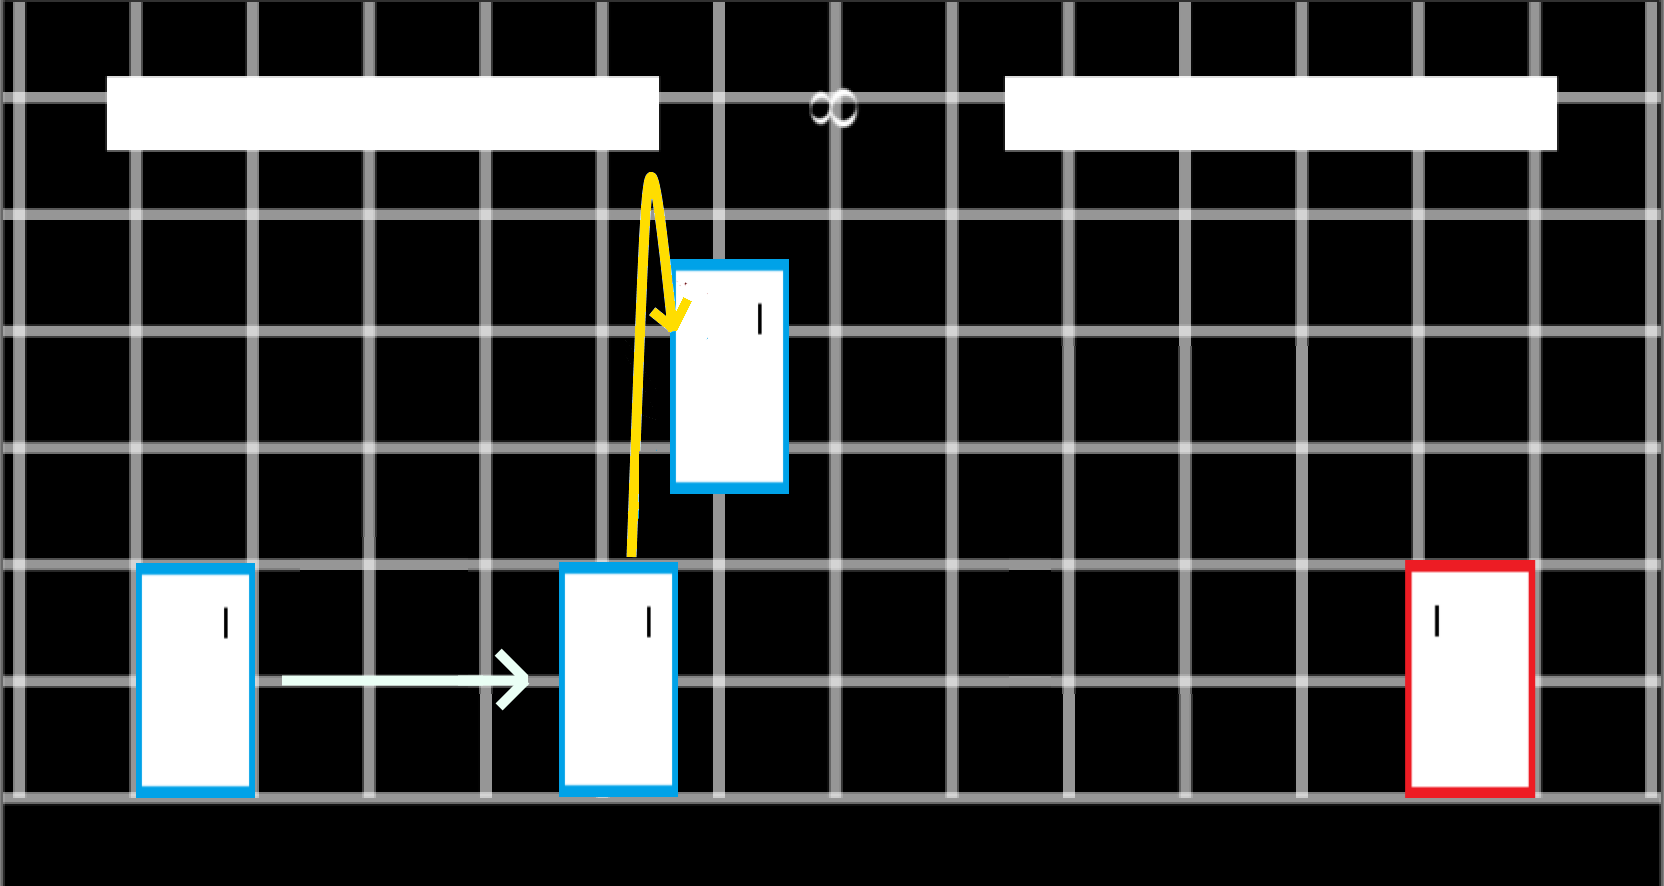
\includegraphics[width=\textwidth]{Figures/Example1.png}
		\caption{case 1}
		\label{}
	\end{subfigure}
	\begin{subfigure}[h]{0.3\textwidth}
		\centering
		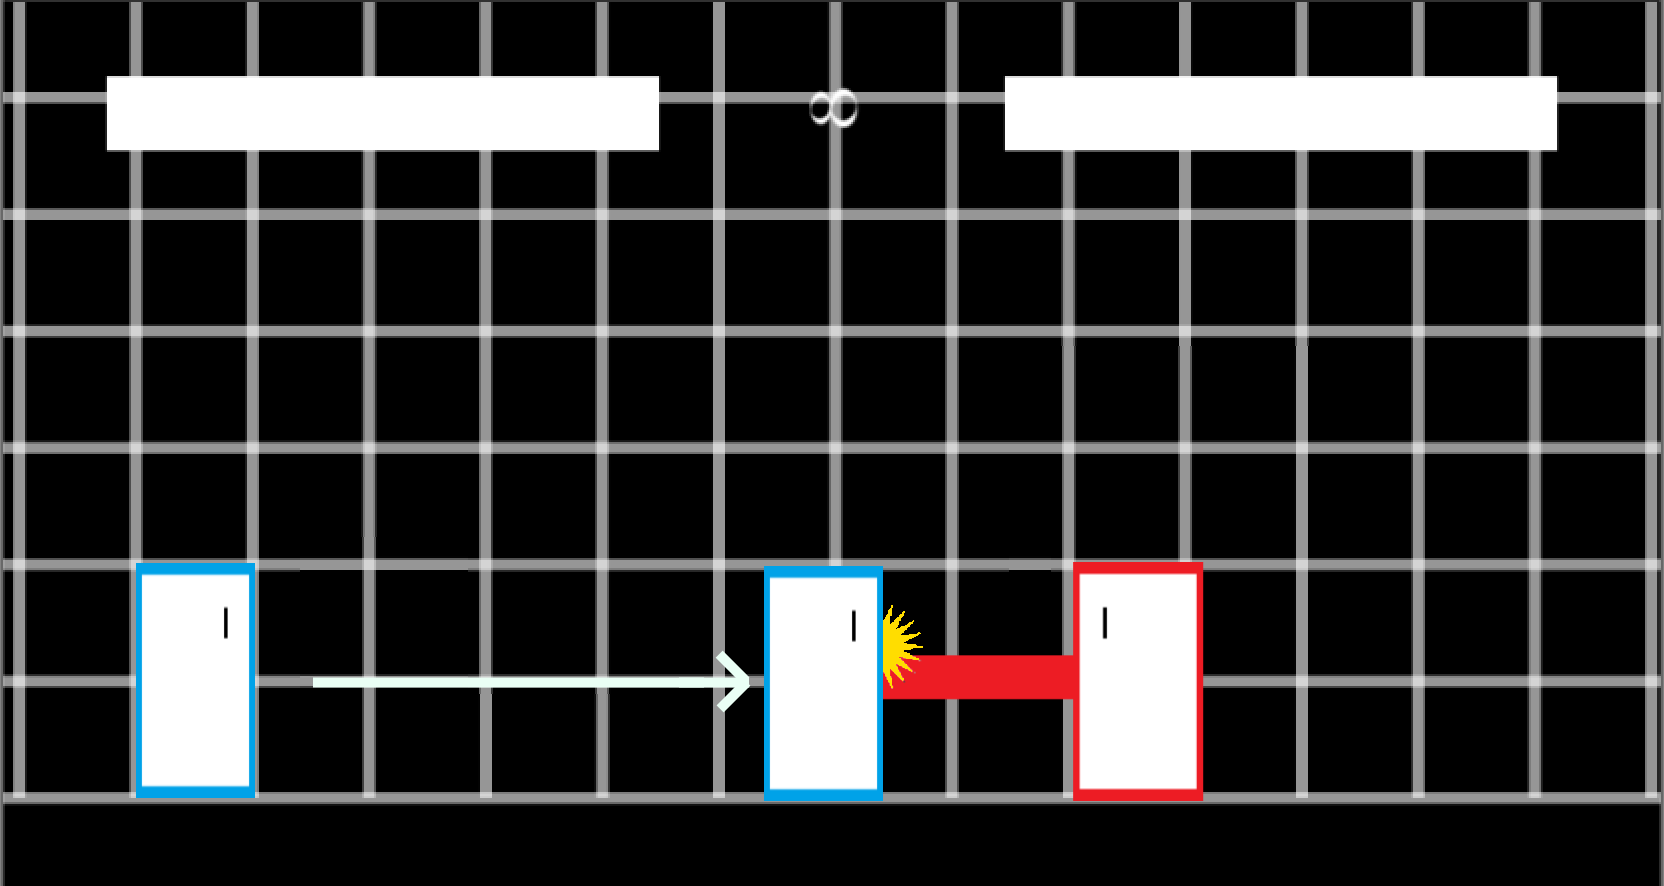
\includegraphics[width=\textwidth]{Figures/Example2.png}
		\caption{case 2}
		\label{}
	\end{subfigure}
	\begin{subfigure}[h]{0.3\textwidth}
		\centering
		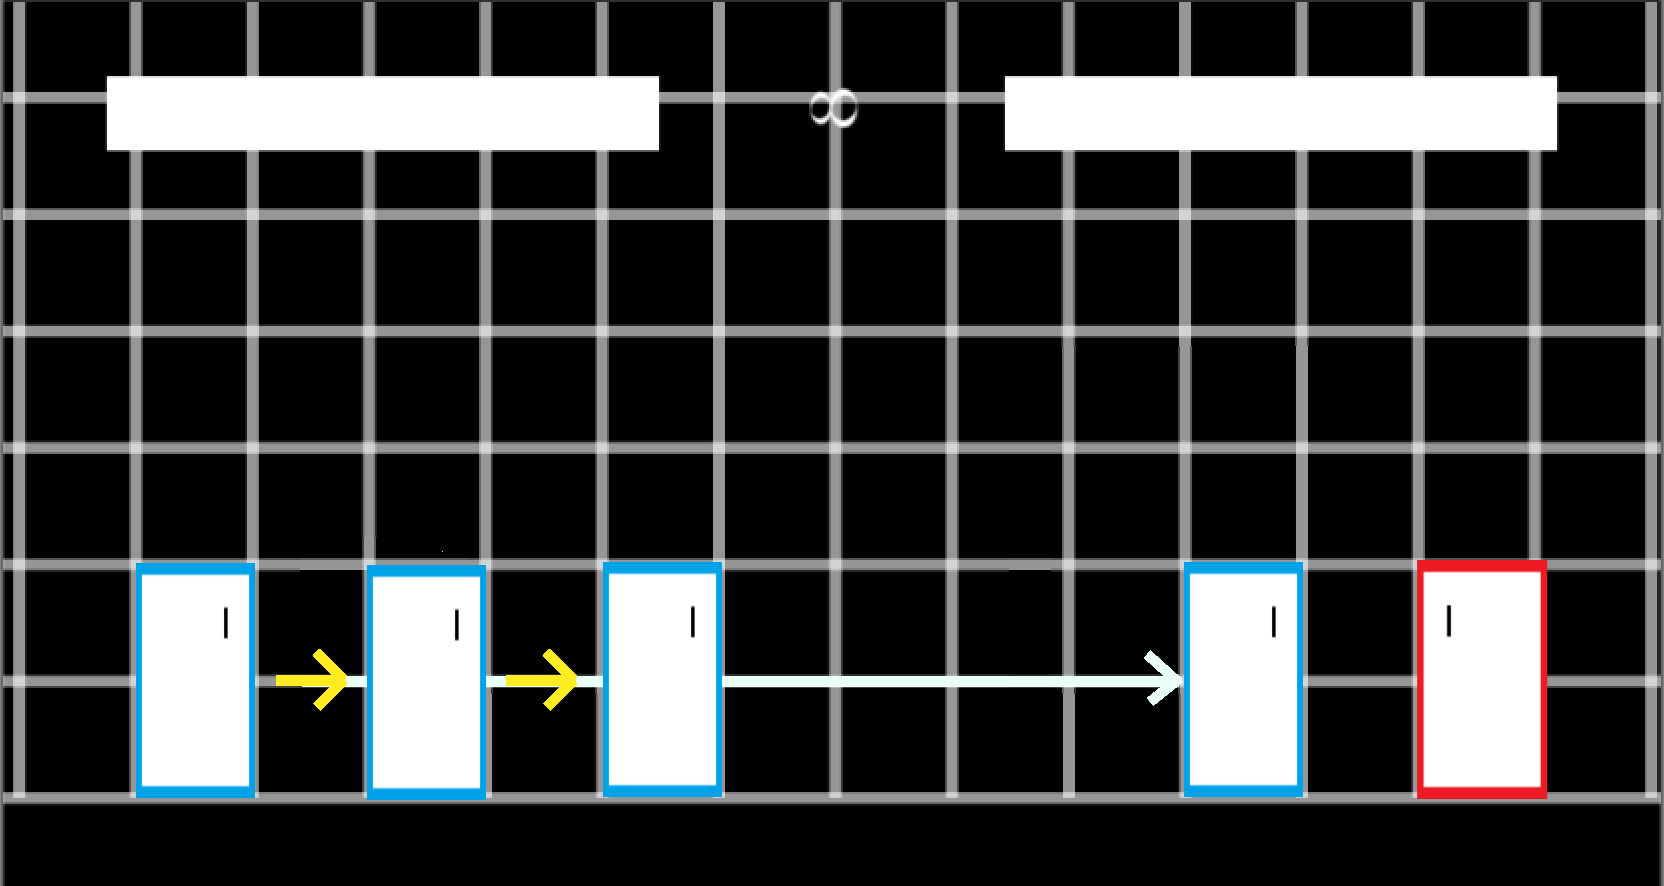
\includegraphics[width=\textwidth]{Figures/Example3.png}
		\caption{case 3}
		\label{}
	\end{subfigure}
\end{figure}

The last case is particularly important for the algorithm, as it breaks down the single player's action of walking forward into multiple smaller component actions that the AI can use.

These transitions are saved as both known-transitions and $\delta$-transitions. All known transitions are stored in a table $K$ where $K[s]$ contains a list of all outgoing transitions $(a,s')$. All $\delta$-transitions are also saved into a table $D$ where $D[a]$ contains all action-$\delta$s encountered. 

An action-$\delta$ is calculated as follows given an observed transition $(s, a, s')$. $p$ represents the target player's state information an $q$ represents the opponent's state information

\begin{table}[h]
	\centering
	\caption{How action-$\delta$ is calculated}
	\begin{tabular}{| c | c | c | c |}
		\hline
		 & $s$ & $s'$ & action-$\delta$ \\
		\hline
		x Position        			& $p_{x}$ & $p_{x}'$ & $p_{x}' - p_{x}$ 	\\
		\hline            			
		y Position        			& $p_{y}$ & $p_{y}'$ & $p_{y}' - p_{y}$ 	\\
		\hline            			
		x Velocity        			& $p_{xVel}$ & $p_{xVel}'$ & $p_{xVel}' - p_{xVel}$  \\
		\hline            			
		y Velocity        			& $p_{yVel}$ & $p_{yVel}'$ & $p_{yVel}' - p_{yVel}$	\\
		\hline
		opponents x Position        & $q_{x}$ & $q_{x}'$ & $q_{x}' - q_{x}$	\\
		\hline
		opponents y Position        & $q_{y}$ & $q_{y}'$ & $q_{y}' - q_{y}$ \\
		\hline
		opponents x Velocity        & $q_{xVel}$& $q_{xVel}$' & $q_{xVel}' - q_{xVel}$	\\
		\hline
		opponents y Velocity        & $q_{yVel}$ & $q_{yVel}'$ & $q_{yVel}' - q_{yVel}$	\\
		\hline
		grounded        			& $p_{grounded}$ & $p_{grounded}'$ & $p_{grounded}'$	\\
		\hline
		opponent grounded       	& $q_{grounded}$ & $q_{grounded}'$ & $q_{grounded}'$ 	\\
		\hline
		status       				& $p_{status}$ & $p_{status}'$ & $p_{status}'$ 	\\
		\hline
		opponents status        	& $q_{status}$ & $q_{status}'$ & $q_{status}'$ 	\\
		\hline
	\end{tabular}
	\label{gamestate}
\end{table}

In the case of the simple demonstration, some of the known-transitions that are extracted are as follows.

\begin{table}[h]
	\centering
	\small
	\caption{Examples of Known-Transitions generated by the demonstration}
	\begin{tabular}{| c | c | c |}
		\hline
		s & a & s' \\
		\hline
		[-6,0,0,0,1,0,0,0,true,true,Stand,Stand] & WalkRight 1 & [-6,0,1,0,1,0,0,0,true,true,Moving,Stand]\\
		\hline
		[-6,0,0,0,1,0,0,0,true,true,Stand,Stand] & WalkRight 10 & [-4,0,1,0,1,0,0,0,true,true,Moving,Stand]\\
		\hline
		[-6,0,0,0,1,0,0,0,true,true,Stand,Stand] & WalkRight 30 & [0,0,1,0,1,0,0,0,true,true,Moving,Stand]\\
		\hline
		[0,0,1,0,1,0,0,0,true,true,Moving,Stand] & Crouch 1 & [0,0,0,0,1,0,0,0,true,true,Crouch,Stand]\\
		\hline
		[0,0,1,0,1,0,0,0,true,true,Crouch,Stand] & JumpNeutral 1 & [0,0,0,1,1,0,0,0,true,false,Air,Stand]\\
		\hline
		[0,0,1,0,1,0,0,0,true,true,Crouch,Stand] & JumpNeutral 45 & [0,0,0,-1,1,0,0,0,true,false,Air,Stand]\\
		\hline
		[0,0,0,-1,1,0,0,0,true,false,Air,Stand] & AirAttack 3 & [0,0,0,-1,1,0,0,0,true,false,AirAttack,FresHit]\\
		\hline
	\end{tabular}
	\label{transitions}
\end{table}

The corresponding action-$\delta$s are then described in table $\ref{delta-transitions}$

\begin{table}[h]
	\centering
	\begin{tabular}{| c | c |}
		\hline
		a & action-$\delta$ \\
		\hline
		WalkRight 1 & [0,0,1,0,0,0,0,0,true,true,Moving,Stand]\\
		\hline
		WalkRight 10 & [2,0,1,0,0,0,0,0,true,true,Moving,Stand]\\
		\hline
		WalkRight 30 & [6,0,1,0,0,0,0,0,true,true,Moving,Stand]\\
		\hline
		Crouch 1 & [0,0,0,0,0,0,0,0,true,true,Crouch,Stand]\\
		\hline
		JumpNeutral 1 & [0,0,0,1,0,0,0,0,true,false,Air,Stand]\\
		\hline
		JumpNeutral 45 & [0,0,0,-1,0,0,0,0,true,false,Air,Stand]\\
		\hline
		Attack 3 & [0,0,0,-1,1,0,0,0,true,false,AirAttack,Freshit]\\
		\hline
	\end{tabular}
	\caption{Examples of Known-Transitions generated by the demonstration}
	\label{delta-transitions}
\end{table}

Lastly, we extract goal-states from the demonstration. These are simply states $s'$ found from the transitions where the opponent's status is \textit{FreshHit}. 

The set of goal states obtained form the demonstration are seen in figure $\ref{goalstates}$

\begin{table}[h]
	\centering
	\begin{tabular}{| c | c | c | c | c | c | c | c | c | c | c | c |}
		\hline
		$p_x$ & $p_y$ & $p_{xVel}$ & $p_{yVel}$ & $q_x$ & $q_y$ & $q_{xVel}$ & $q_{yVel}$ & $p_{grounded}$ & $q_{grounded}$ & $p_{status}$ & $q_{status}$\\
		\hline
		0 & 0 & 0 & 0 & 0 & 0 & 0 & 0 & true & true & LowAttack & FreshHit\\
		\hline
		0 & 0 & 0 & -1 & 1 & 0 & 0 & 0 & true & true & AirAttack & FreshHit\\
		\hline
	\end{tabular}
	\caption{Goal states generated by the demonstration}
	\label{goalstates}
\end{table}


\subsection{Generating Successors}

When generating a successor using a known-transition, the successor is the same $s'$ as the one observed during the demonstration. By traveling along known successors, the plan generated by the search closely follows the exact actions taken by the player during demonstration

%\begin{figure}[h]
%	\centering
%	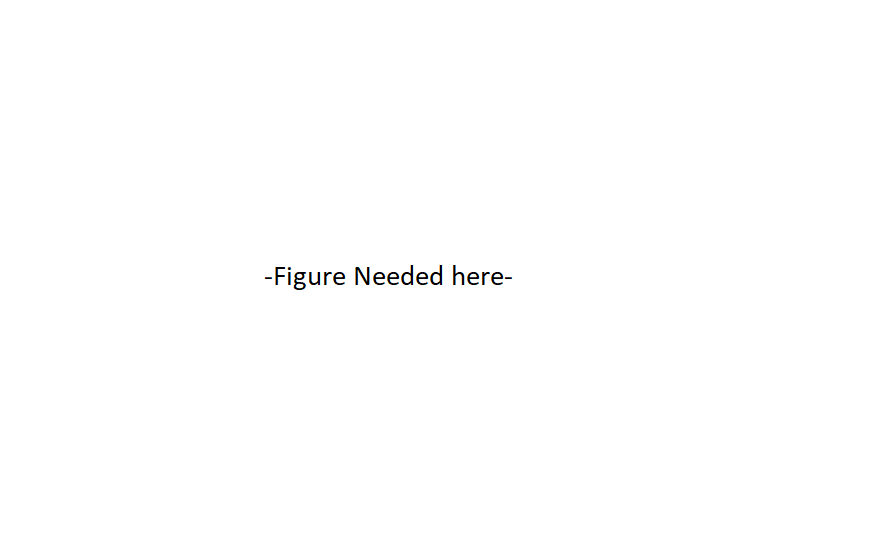
\includegraphics[width=\textwidth]{Figures/Placeholder.png}
%	\caption{The AI follows the player's demonstration}
%	\label{followdemonstration}
%\end{figure}

When generating a successor using $\delta$-transitions, we rely on a predictor function $\phi(s,a)$. The predictor works as follows.

To determine the effect of taking action $a$, we look at all action-$\delta$s associated with action $a$. We will refer to these action-$\delta$'s as $\delta$. Each $\delta$ has a \textit{prior} called $s_{\delta}$, which indicates the starting state of that particular recorded transition. We can assign a similarity score between the $s$ and $s_{\delta}$, which we use as a rough approximation of our confidence in the truth of that action.

$$sim(s, s_{\delta}) = 1-\frac{\sum_i dist(s[i], s_{\delta}[i])}{\sum_i max_i}$$

$$dist(s[i], s_{\delta}[i]) =
\begin{cases}
s_{\delta}[i] - s[i] & \text{if $i$ represents the x position of either player} \\
s_{\delta}[i] == s[i] & \text{otherwise}
\end{cases}
$$

$s[i]$ represents the value of field $i$ in state $s$ and $max_[i]$ represents the maximum value of $dist(s[i], s_{\delta}[i])$. 

We then create a predicted action-$\delta$ by taking a weighted average over the action-$\delta$s and the similarity score and then rounding the result.

$$\delta^*[i] \approx
\begin{cases}
argmax_\delta \frac{sim(s, s_{\delta})}{\sum_\delta sim(s, s_{\delta})}[i] & \text{if $s[i]$ is a categorical variable} \\
\sum_\delta \frac{sim(s, s_{\delta}) \delta[i] }{\sum_\delta sim(s, s_{\delta})} & \text{otherwise}
\end{cases}
$$

To get the final prediction, we apply $\delta^*$ to the current state $s$ to get $s'$.

The confidence value $c$ that is returned with this prediction is calculated as follows.

$$c = sim(s, s_{\delta}) \text{ where } \delta = argmax_\delta \frac{sim(s, s_{\delta})}{\sum_\delta sim(s, s_{\delta})}$$

This represents our belief in the predicted result and it also gives an indication of likelihood that the player would take this action.

%With the model of the game dynamics, we can then begin to compute the successors of state $s$. There are two cases that we differentiate between.

%\textbf{Case 1: Known states}
%If $s$ is a state that was encountered in the demonstration, then we have precise knowledge of the player's behavior in that state. Specifically, $T[s]$ contains all of actions $A$ that the player has taken at that state. To best model the player the AI restricts itself to taking the same kinds of actions that the player has in those states, so it only adds $succ(s,a)$ where $a \in A$. In addition, we have good predictions for the value of $s' = succ(s,a)$ since we have the transitions $(s,a,s')$ stored within $T$.

%==========Insert example of the simple look up here============

%\textbf{Case 2: Unknown states}
%The AI is likely to see states which were not seen during the demonstration. In this case, we have no clear basis for knowing what the target player would do. 

%In this case, we first determine the types of actions that are valid in the AI's current state. This rules out using impossible actions, such as walking forward while the AI is airborne. From the remaining action types, we look at all valid actions $a$ from the demonstration and predict the result of taking that action.

%Specifically, the predictor is works as follows. To determine the effect of taking performed action $a$, we look at $D[a]$. We then do a weighted average over all of $\Delta_a$ to derive the final prediction. The weighting is set according to the similarities of the prior states for each action effect.

\subsection{Costs}

In order to differentiate the qualities of plans, we need a suitable cost function. The cost of taking a known-transition is 1, as there is no qualitative way to evaluate one demonstrated action as being more "human-like" than another. For a $\delta$-transitions, we apply an additional penalty that is inversely proportional to the confidence returned by the predictor.

$$(s',c) = \phi(s, a)$$
$$Cost(s, s') = \lambda/c$$

Where $\lambda$ is a hypervariable. This makes it so that shorter plans which use higher confidence transitions are preferred. 

\subsection{The Goal and Heuristics}

Before beginning the search, we select a random goal state from the demonstration to target. This the goal states selected are weighted by their similarity to the initial starting state. This goal state has certain qualities that are important to target. Namely, we care about the distance between the player and the opponent and the status of the player and opponent. The search tries form a plan that results in a state which matches these qualities. 

In order to efficiently guide the search towards such a state, we reduce the current state to these qualities. The heuristic we use is then a measure the total distance between the current state's qualities and the goal state's qualities. The quality of a state is shown in the below table.

\begin{table}[h]
	\centering
	\caption{The qualities extracted from state $s$}
	\begin{tabular}{| c | c | c | c |}
		\hline
		Field Name & Value\\
		\hline
		x Distance        			& $|p_x - q_x|$ \\
		\hline            			
		y Distance        			& $|p_y - q_y|$ 	\\
		\hline
		grounded        			& $p_{grounded}$ \\
		\hline
		opponent grounded       	& $q_{grounded}$ \\
		\hline
		status       				& $p_{status}$ \\
		\hline
		opponents status        	& $q_{status}$ \\
		\hline
	\end{tabular}
	\label{qualities}
\end{table}

%\section{Goal states and Heuristics}
%The final component we need to effectively perform search in this space is a goal state and heuristic function. 

%Because our objective is to have the AI exhibit a certain kind of behavior, the goal state is only partially-specified. The function \textit{IsGoal()} determines whether a state is a goal state and is designed as follows.

%Firstly, because this AI is intended to provide competitive players an more authentic representation of human play, the considered state must have the opponent in the \textit{FirstHit} status. Additionally, human players mix up their short-term strategies for getting hits so that they aren't predictable. To emulate this characteristic, we randomly select an instance in our demonstration where the opponent has the \textit{FirstHit} status and designate that as the \textbf{target}. We then require that the considered state has qualities similar to the target. This refers to the relative positions of the players and characteristics of each player's behavior states. 

%For the heuristic, when evaluating state $s$, we took the Manhattan Distance of the relative positions of the 2 players and added that to the number of other parameters in $s$ which do not match the values in the target state $t$.

%This \textbf{IsGoal()} function and the heuristic then gives us the following kind of behavior.

%\begin{figure}[t]
%	\centering
%	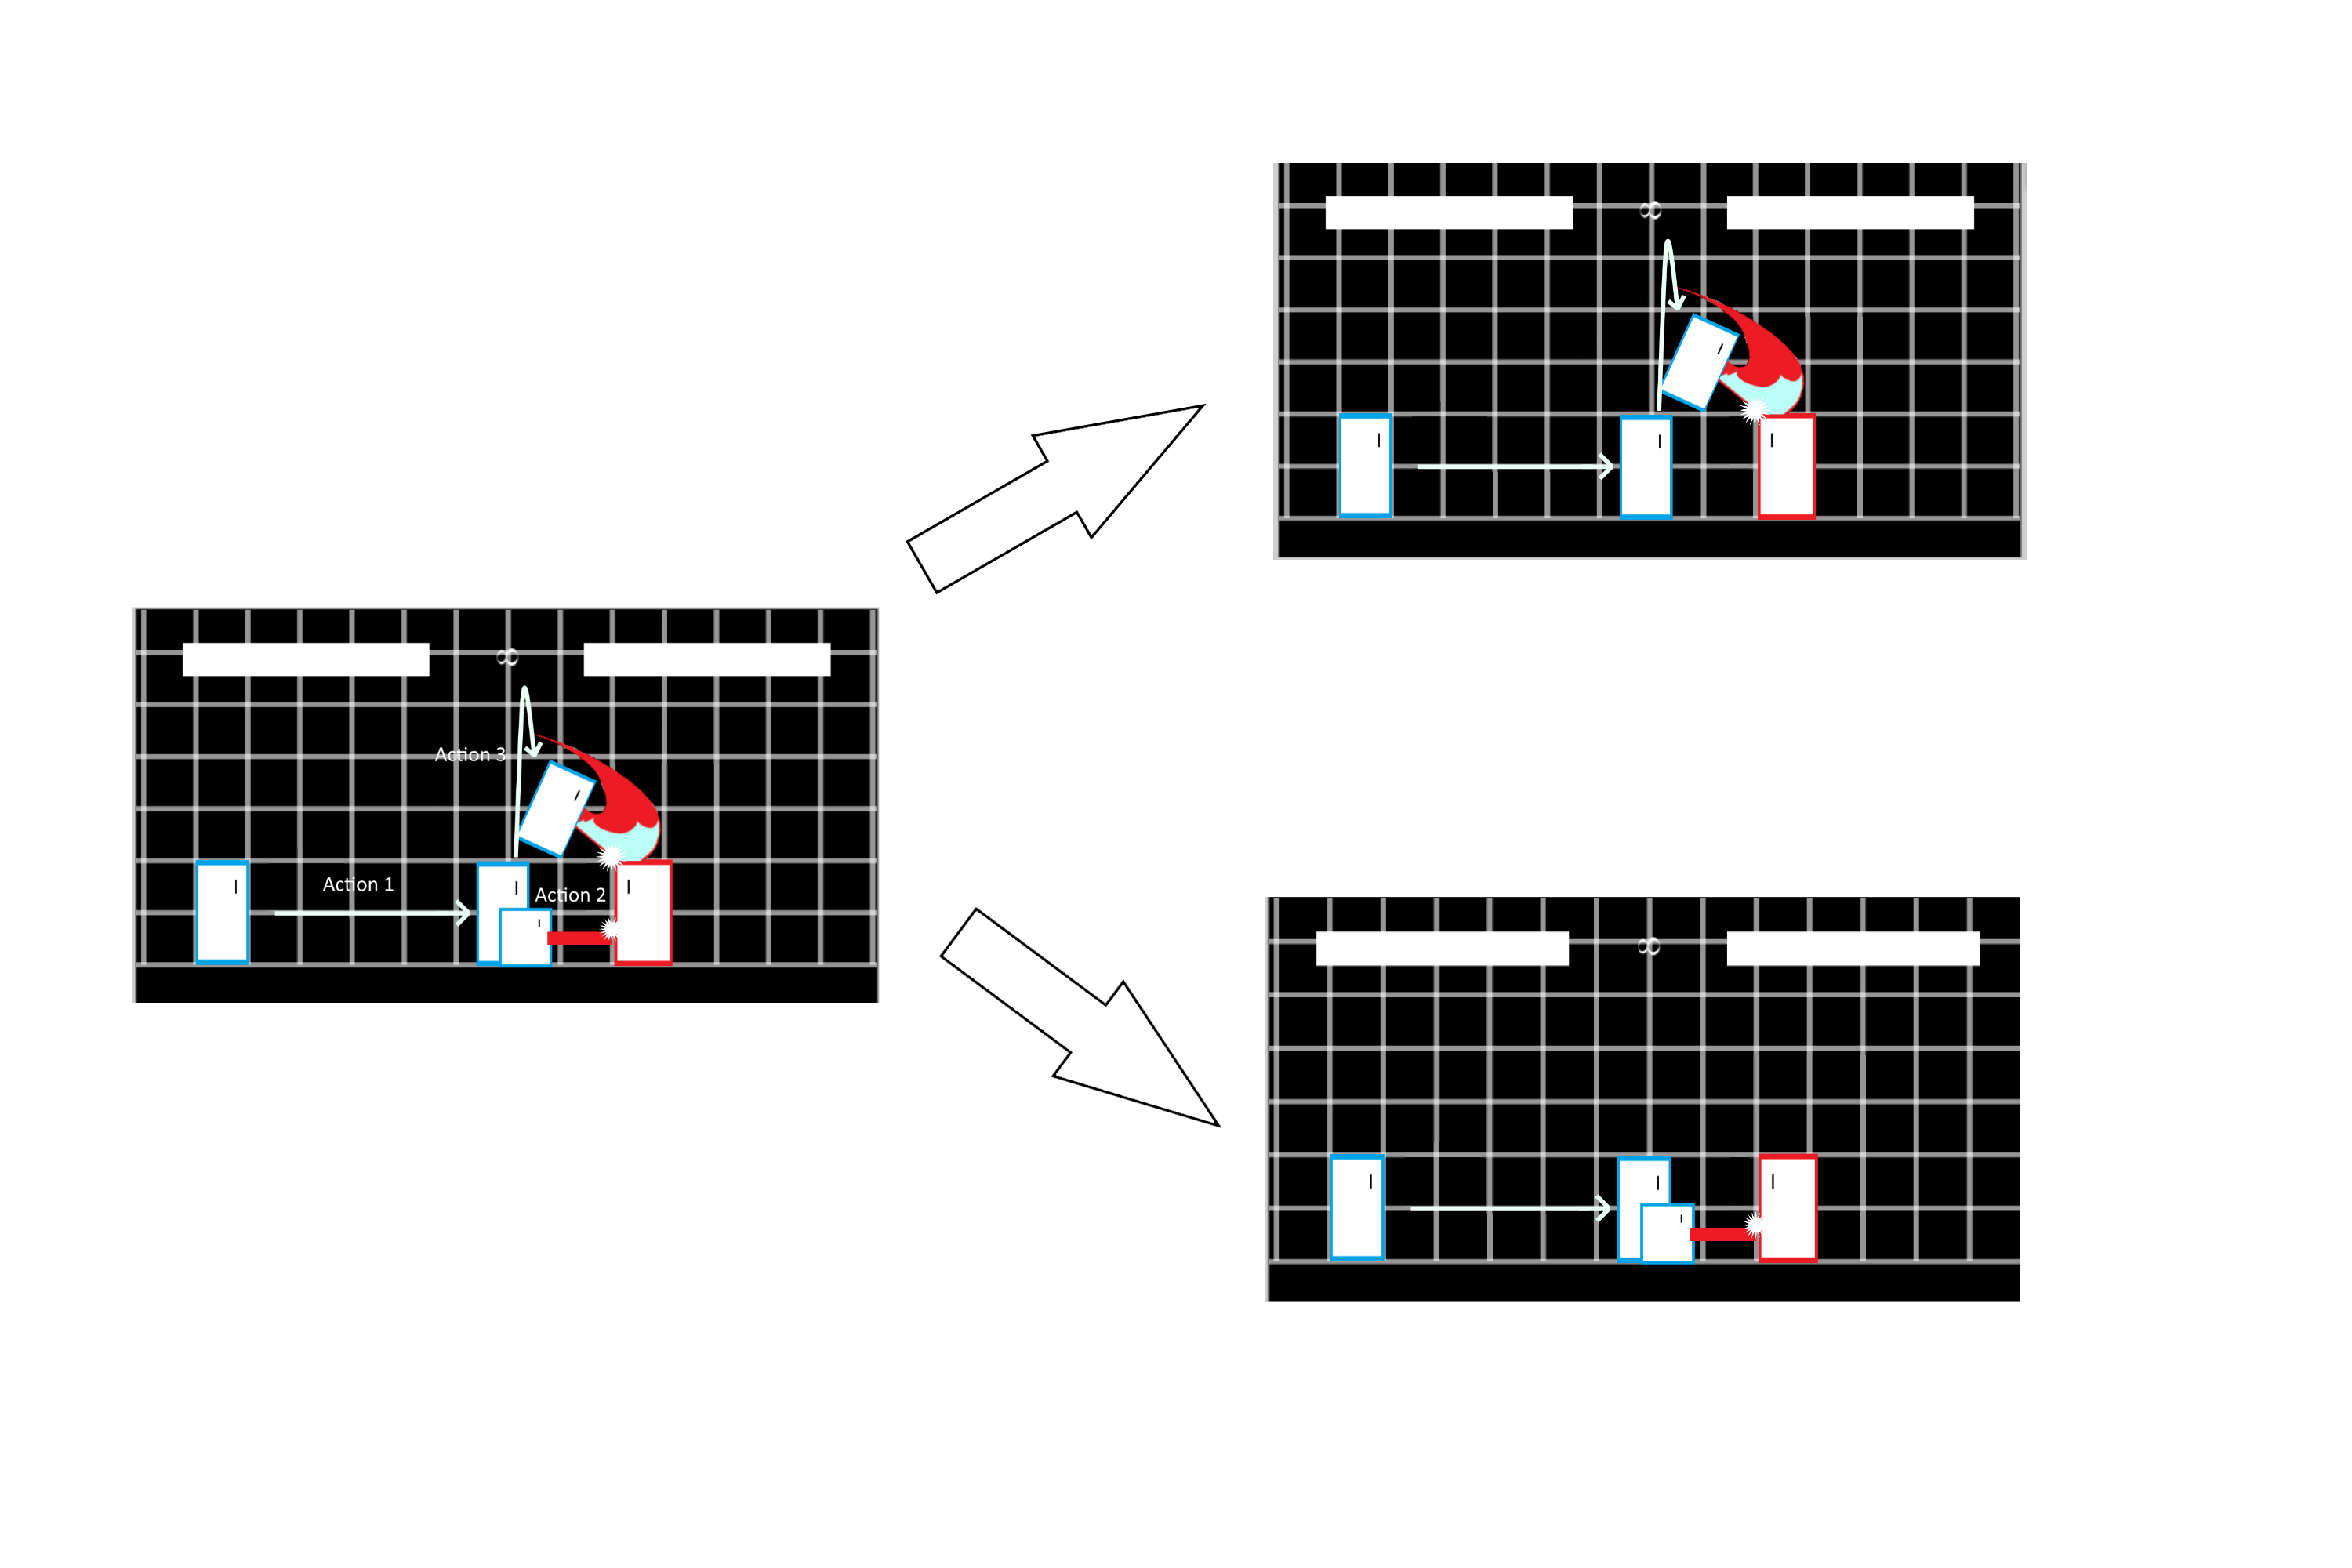
\includegraphics[width=\textwidth]{Figures/DecisionMaking.png}
%	\caption{Action Effects}
%	\label{ActionEffects}
%\end{figure}

%In the demonstration, we have one instance where the player hits the opponent with a low attack and another instance where the player hits the opponent with a jumping attack. One of the instances is randomly selected to be the target, and the AI then follows the appropriate plan to execute.

\section{Additional Considerations}

\subsection{Dealing with long search times: Anytime Search}
Because of fast-paced nature of fighting games, players need to be able to reliably make split second decisions. This constraint then extends to our AI, as it can't afford to plan seconds at a time, as the game state might change drastically within that time period. In our implementation, the AI is required to come up with a plan within 50 milliseconds. If it cannot reach a goal state, it instead formulates a plan to get to the state with the highest projected value. The idea is that by reaching this intermediate state, it can then resume plannning from the position that is closer to the goal, giving the impression of one seemless plan, when it in fact generated that plan during execution.

%\begin{figure}[h]
%	\centering
%	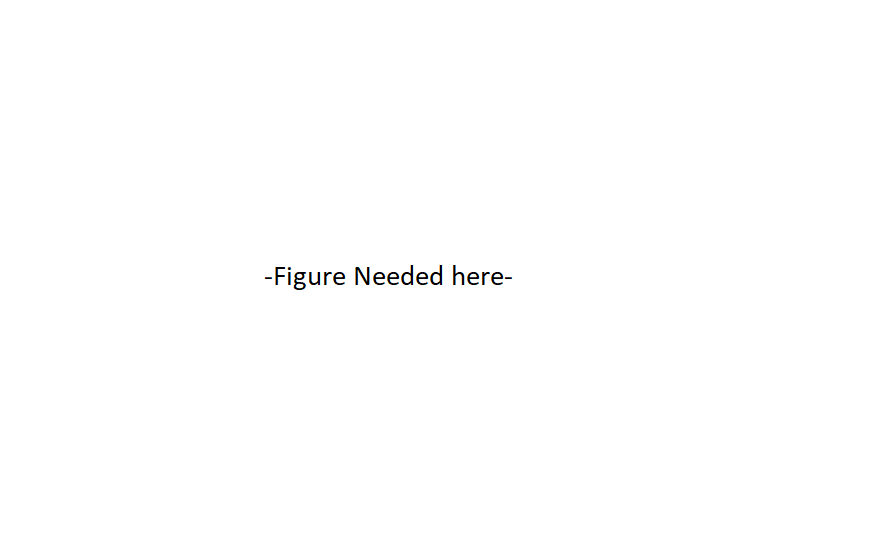
\includegraphics[width=\textwidth]{Figures/Placeholder.png}
%	\caption{The AI finds the best available state}
%	\label{anytime}
%\end{figure}

\subsection{Dealing with a changing game state: replanning}
Because the opponent is allowed to move during plan execution, the plan we formulate is likely to encounter a state that we didn't expect. Because of the short time to plan we enforced, we can seemlessly replan whenever we hit an unexpected state and have the AI adjust accordingly. An example of this is when the opponent moves back while the AI is approaching them. Due to replanning, the AI will then know to continue to move towards the opponent, rather than stopping at it's original location and attacking like initially planned.

%\begin{figure}[h]
%	\centering
%	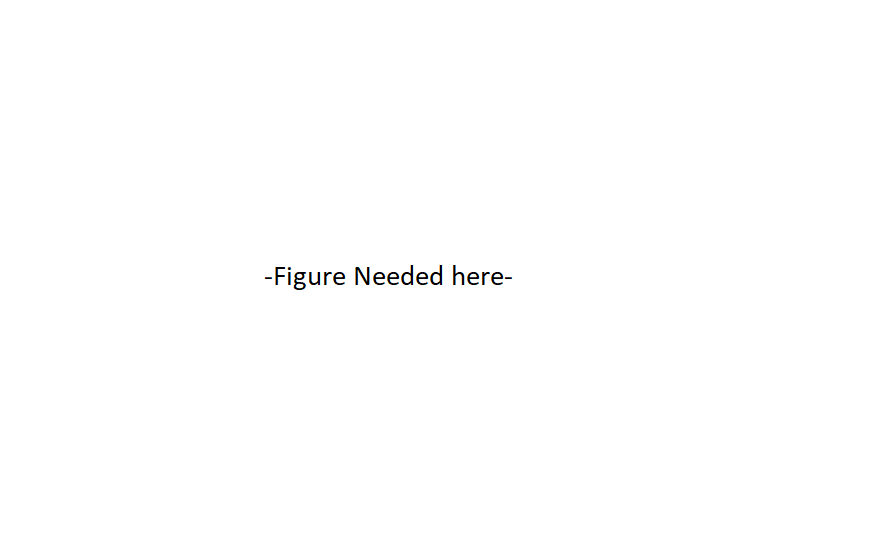
\includegraphics[width=\textwidth]{Figures/Placeholder.png}
%	\caption{The AI quickly forms a new plan}
%	\label{replanning}
%\end{figure}

\subsection{Dealing with bad predictions, updating the predictor}
One final thing that we do to ensure that our AI is robust is update the predictor. As the game progresses, the AI logs the transitions that don't match up with its predictions and adds it back to the training set. This helps the AI make better predictions in the future and helps avoid local minima plans. This is crucially important as otherwise the AI is likely to get stuck performing the same action repeatedly.

Talking about the search here

\section{action-$\delta$s}
First, we explain the concept of action-$\delta$s, which our work relies on. When a player takes action $a$ from state $s$ and arrives at state $s'$, the game state changes because of $a$. For example, the action of walking to the right causes the player's $x$-position to increase. We refer to this change in the game state as an action-$\delta$, which represents how the game state changes as a result of taking action $a$. 

\begin{figure}[t]
	\centering
	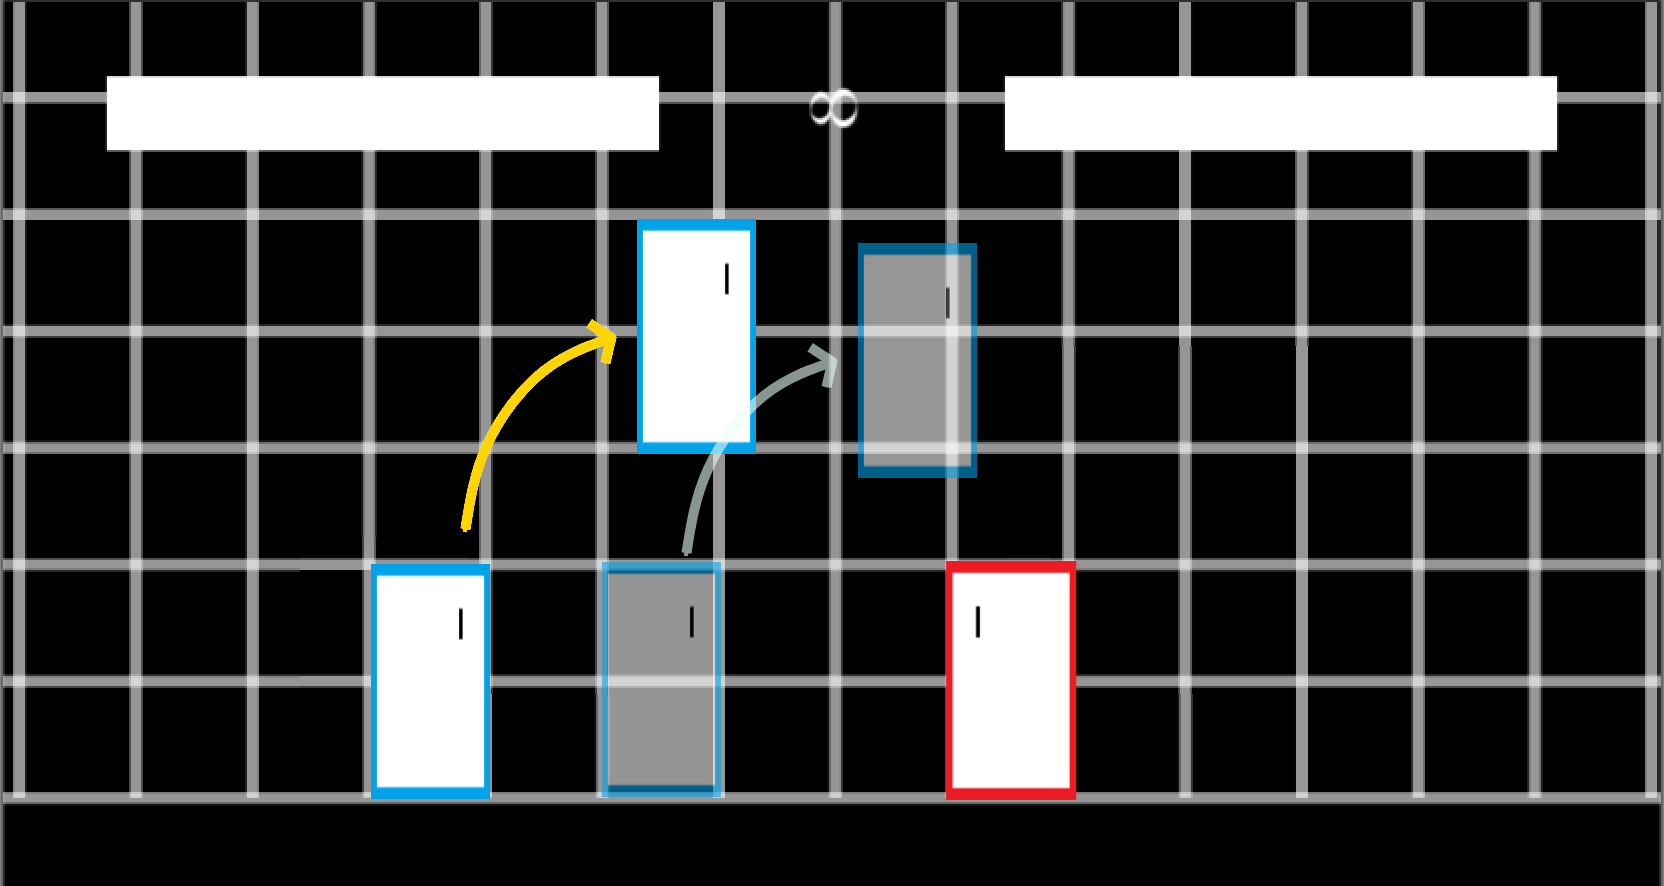
\includegraphics[width=\textwidth]{Figures/ActionDelta.png}
	\caption{Jumping to the right has an action-$\delta$ that puts the player up and to the right}
	\label{}
\end{figure}

These action-$\delta$s are used to understand and build a model of the game's dynamics. If we know how an action affects the game state in one situation, we can predict how the action will affect the game state in similar situation. 

\section{Demonstration $\delta$-Search}
The task of emulating a player's behavior is represented as a graph search problem. Specifically, the objective is to form a plan to hit the opponent using the actions demonstrated by the target player. The plan should be feasible and resemble a plan executed by the target player as much possible.

The search space is represented as graph $G = (V, E)$. The vertices $V$ of the graph are the various states of the game. The edges $E$ represent the possible transitions between game states. 

The transitions that we search on are generated from the training data and fall into two classes. The first class, known-transitions, are tuples $(s,a,s')$ which are identical to ones captured from the demonstration. The other class of transitions are referred to as $\delta$-transitions. These transitions are of the form $(s, a, \phi(s, a))$, where $\phi(s, a)$ is a predictor function that takes in the current state $s$ and an action $a$ performed by the target player. This predictor function generates the predictions by learning from the action-$\delta$s of action $a$ that were obtained from the training data.

Since we want to form a plan that hits the opponent, a valid goal state is one where the opponent has the "FirstHit" status. During a run of the search, the goal is defined to be a state that has the same characteristics as a goal state selected from the demonstration. The goal state is selected according to a weighted distribution. This ensures that the planner's ultimate objective matches that of the target player.

When searching for a feasible plan to get to the goal, we use a modified version of heuristic graph search. We maintain two priority queues throughout the search, one called KNOWN and another called UNKNOWN. When deciding to expand a state, we prioritize expanding states in KNOWN. These states are states which have been seen in the demonstration, which allows us to use the known-transitions to generate the successor states. If there are no states in KNOWN, then we expand states from UNKNOWN using the $\delta$-transitions. After expanding a state, all successors states which have not been expanded by $\delta$-transitions are added to the UNKNOWN priority queue. If a state has been seen in the demonstration and it has not yet been expanded by known-transitions, it is added to the KNOWN priority queue.

\begin{figure}[t]
	\centering
	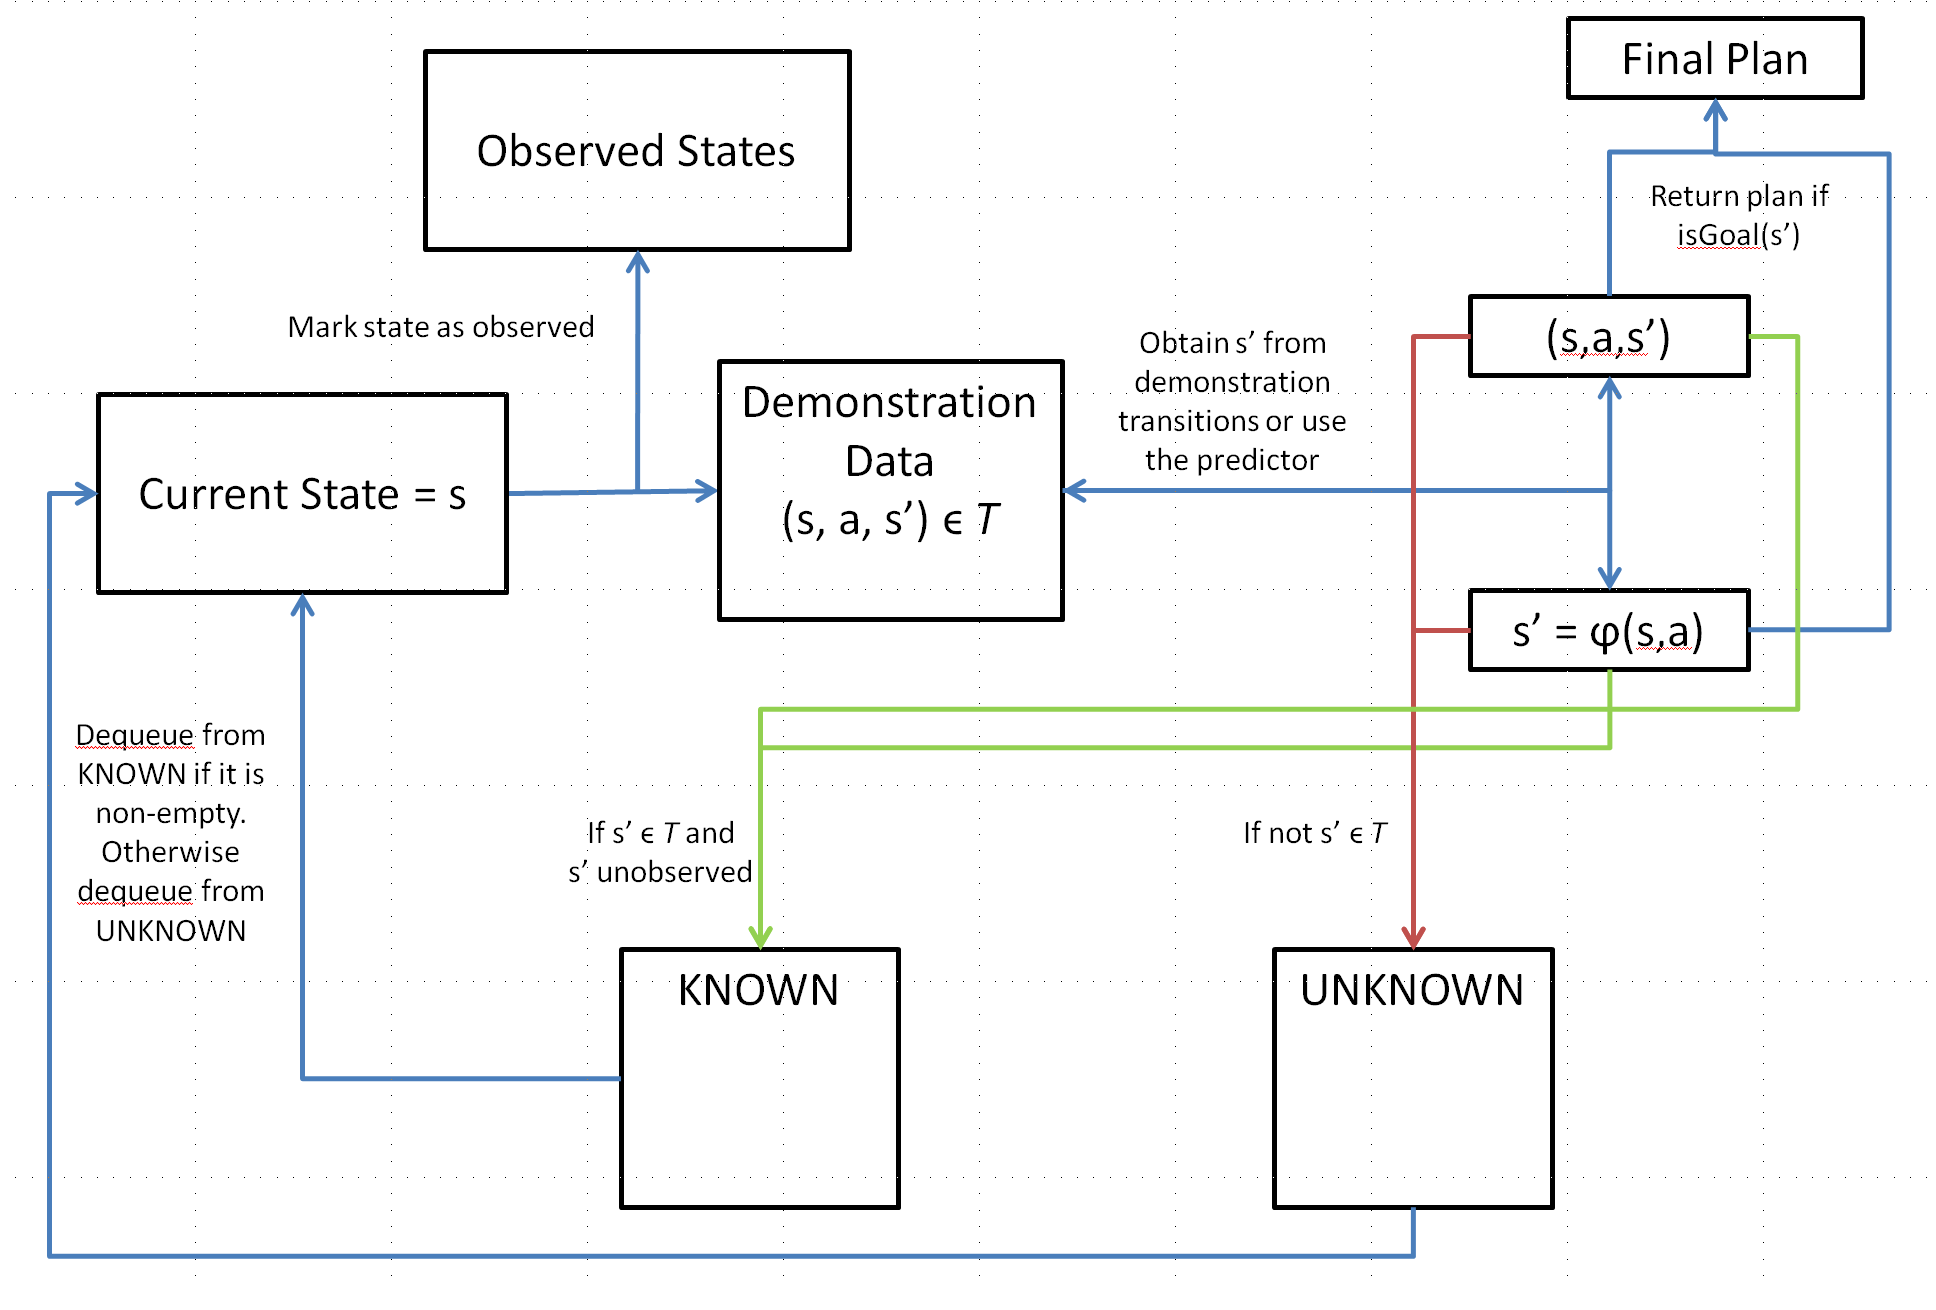
\includegraphics[width=\textwidth]{Figures/SearchSpecificFlowchart.png}
	\caption{Overview of $\delta$-search}
	\label{}
\end{figure}

\section{Pseudo-code}

\begin{algorithm}
	\begin{algorithmic}[1]
		\Function{$\delta$-search($s_{start}, demonstrations$)} {}
		\State $OBS = \{\}$
		\State $OBS_{\delta} = \{\}$
		\State $KNOWN = \{\}$
		\State $UNKNOWN = \{\}$
		\State $s_{goal} = GetGoal(demonstrations)$
		\If {$(s_{start}, \_, \_) \in demonstrations$}
			\State $KNOWN \cup \{s_{start}\}$
		\Else
			\State $UNKNOWN \cup \{s_{start}\}$
		\EndIf
		
		\While {$|KNOWN| \not = 0$ OR $|UNKNOWN| \not = 0$}:
			\If {$|KNOWN| \not = 0$}
				\State Remove the smallest $[f(s) = g(s) + h(s)]$ from $KNOWN$
				\State $OBS \cup \{s\}$
				\If {$isGoal(s)$}	return $plan(s)$ 
				\EndIf
				\State Expand $s$ with $(s,a,s') \in demonstrations$ \hfill $s' \not \in OBS$ OR $s' \not \in OBS_{\delta}$
				\If {$(s', \_, \_) \in demonstrations$}
					\State $KNOWN \cup \{s'\}$
				\EndIf
				\State $UNKNOWN \cup \{s'\}$
			\ElsIf{$|UNKNOWN| \not = 0$}
				\State Remove the smallest $[f(s) = g(s) + h(s)]$ from $UNKNOWN$
				\If {$isGoal(s)$}	return $plan(s)$
				\EndIf
				\State $OBS_{\delta} \cup \{s\}$
				\State Expand $s$ with $s' = \phi(s,a)$ \hspace{2cm}  $s' \not \in OBS$ OR $s' \not \in OBS_{\delta}$
				\If {$(s', \_, \_) \in demonstrations$}
					\State $KNOWN \cup \{s'\}$
				\EndIf
				\State $UNKNOWN \cup \{s'\}$	
			\EndIf
		\EndWhile
		\EndFunction
	\end{algorithmic}
\end{algorithm}

%Incorporate the reasoning into the description

%\section{Reasoning}

%The reason we keep two separate priority queues is to encourage the AI to follow the demonstration before trying to explore situations that it hasn't seen before. This is both because of the reduced branching factor of following the demonstration and because following the demonstration of a human-player is inherently more human-like and less-likely to have unexpected outcomes.

%To form a feasible strategy to get from from start state $s_{start}$ to a set of goal states $S_{goal}$, we use heuristic graph search. We first add $s = s_{start}$ to a priority queue with priority $g(s) + h(s)$, where $g(s)$ is the minimum cost to reach that state (0 in the case of $s_{start}$)and $h(s)$ is our heuristic estimate for the cost of getting from $s$ to a goal state. We then dequeue the state $s$ with the lowest cost from the priority queue. If it is a goal state, we stop and return the corresponding plan. If it is not, we repeat the process, inserting $s' = succ(s, a)$ into the priority queue with the appropriate priority, given  that we have not seen $s'$ before.

%\section{Justification and Objectives}
